\documentclass[1p]{elsarticle_modified}
%\bibliographystyle{elsarticle-num}

%\usepackage[colorlinks]{hyperref}
%\usepackage{abbrmath_seonhwa} %\Abb, \Ascr, \Acal ,\Abf, \Afrak
\usepackage{amsfonts}
\usepackage{amssymb}
\usepackage{amsmath}
\usepackage{amsthm}
\usepackage{scalefnt}
\usepackage{amsbsy}
\usepackage{kotex}
\usepackage{caption}
\usepackage{subfig}
\usepackage{color}
\usepackage{graphicx}
\usepackage{xcolor} %% white, black, red, green, blue, cyan, magenta, yellow
\usepackage{float}
\usepackage{setspace}
\usepackage{hyperref}

\usepackage{tikz}
\usetikzlibrary{arrows}

\usepackage{multirow}
\usepackage{array} % fixed length table
\usepackage{hhline}

%%%%%%%%%%%%%%%%%%%%%
\makeatletter
\renewcommand*\env@matrix[1][\arraystretch]{%
	\edef\arraystretch{#1}%
	\hskip -\arraycolsep
	\let\@ifnextchar\new@ifnextchar
	\array{*\c@MaxMatrixCols c}}
\makeatother %https://tex.stackexchange.com/questions/14071/how-can-i-increase-the-line-spacing-in-a-matrix
%%%%%%%%%%%%%%%

\usepackage[normalem]{ulem}

\newcommand{\msout}[1]{\ifmmode\text{\sout{\ensuremath{#1}}}\else\sout{#1}\fi}
%SOURCE: \msout is \stkout macro in https://tex.stackexchange.com/questions/20609/strikeout-in-math-mode

\newcommand{\cancel}[1]{
	\ifmmode
	{\color{red}\msout{#1}}
	\else
	{\color{red}\sout{#1}}
	\fi
}

\newcommand{\add}[1]{
	{\color{blue}\uwave{#1}}
}

\newcommand{\replace}[2]{
	\ifmmode
	{\color{red}\msout{#1}}{\color{blue}\uwave{#2}}
	\else
	{\color{red}\sout{#1}}{\color{blue}\uwave{#2}}
	\fi
}

\newcommand{\Sol}{\mathcal{S}} %segment
\newcommand{\D}{D} %diagram
\newcommand{\A}{\mathcal{A}} %arc


%%%%%%%%%%%%%%%%%%%%%%%%%%%%%5 test

\def\sl{\operatorname{\textup{SL}}(2,\Cbb)}
\def\psl{\operatorname{\textup{PSL}}(2,\Cbb)}
\def\quan{\mkern 1mu \triangleright \mkern 1mu}

\theoremstyle{definition}
\newtheorem{thm}{Theorem}[section]
\newtheorem{prop}[thm]{Proposition}
\newtheorem{lem}[thm]{Lemma}
\newtheorem{ques}[thm]{Question}
\newtheorem{cor}[thm]{Corollary}
\newtheorem{defn}[thm]{Definition}
\newtheorem{exam}[thm]{Example}
\newtheorem{rmk}[thm]{Remark}
\newtheorem{alg}[thm]{Algorithm}

\newcommand{\I}{\sqrt{-1}}
\begin{document}

%\begin{frontmatter}
%
%\title{Boundary parabolic representations of knots up to 8 crossings}
%
%%% Group authors per affiliation:
%\author{Yunhi Cho} 
%\address{Department of Mathematics, University of Seoul, Seoul, Korea}
%\ead{yhcho@uos.ac.kr}
%
%
%\author{Seonhwa Kim} %\fnref{s_kim}}
%\address{Center for Geometry and Physics, Institute for Basic Science, Pohang, 37673, Korea}
%\ead{ryeona17@ibs.re.kr}
%
%\author{Hyuk Kim}
%\address{Department of Mathematical Sciences, Seoul National University, Seoul 08826, Korea}
%\ead{hyukkim@snu.ac.kr}
%
%\author{Seokbeom Yoon}
%\address{Department of Mathematical Sciences, Seoul National University, Seoul, 08826,  Korea}
%\ead{sbyoon15@snu.ac.kr}
%
%\begin{abstract}
%We find all boundary parabolic representation of knots up to 8 crossings.
%
%\end{abstract}
%\begin{keyword}
%    \MSC[2010] 57M25 
%\end{keyword}
%
%\end{frontmatter}

%\linenumbers
%\tableofcontents
%
\newcommand\colored[1]{\textcolor{white}{\rule[-0.35ex]{0.8em}{1.4ex}}\kern-0.8em\color{red} #1}%
%\newcommand\colored[1]{\textcolor{white}{ #1}\kern-2.17ex	\textcolor{white}{ #1}\kern-1.81ex	\textcolor{white}{ #1}\kern-2.15ex\color{red}#1	}

{\Large $\underline{11a_{223}~(K11a_{223})}$}

\setlength{\tabcolsep}{10pt}
\renewcommand{\arraystretch}{1.6}
\vspace{1cm}\begin{tabular}{m{100pt}>{\centering\arraybackslash}m{274pt}}
\multirow{5}{120pt}{
	\centering
	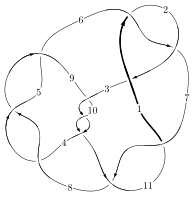
\includegraphics[width=112pt]{../../../GIT/diagram.site/Diagrams/png/472_11a_223.png}\\
\ \ \ A knot diagram\footnotemark}&
\allowdisplaybreaks
\textbf{Linearized knot diagam} \\
\cline{2-2}
 &
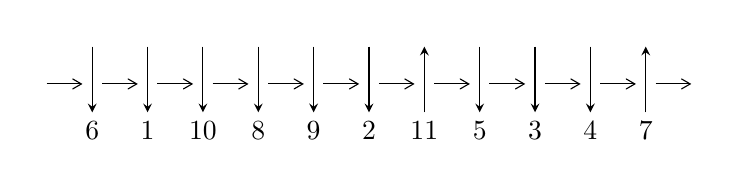
\begin{tikzpicture}[x=20pt, y=17pt]
	% nodes
	\node (C0) at (0, 0) {};
	\node (C1) at (1, 0) {};
	\node (C1U) at (1, +1) {};
	\node (C1D) at (1, -1) {6};

	\node (C2) at (2, 0) {};
	\node (C2U) at (2, +1) {};
	\node (C2D) at (2, -1) {1};

	\node (C3) at (3, 0) {};
	\node (C3U) at (3, +1) {};
	\node (C3D) at (3, -1) {10};

	\node (C4) at (4, 0) {};
	\node (C4U) at (4, +1) {};
	\node (C4D) at (4, -1) {8};

	\node (C5) at (5, 0) {};
	\node (C5U) at (5, +1) {};
	\node (C5D) at (5, -1) {9};

	\node (C6) at (6, 0) {};
	\node (C6U) at (6, +1) {};
	\node (C6D) at (6, -1) {2};

	\node (C7) at (7, 0) {};
	\node (C7U) at (7, +1) {};
	\node (C7D) at (7, -1) {11};

	\node (C8) at (8, 0) {};
	\node (C8U) at (8, +1) {};
	\node (C8D) at (8, -1) {5};

	\node (C9) at (9, 0) {};
	\node (C9U) at (9, +1) {};
	\node (C9D) at (9, -1) {3};

	\node (C10) at (10, 0) {};
	\node (C10U) at (10, +1) {};
	\node (C10D) at (10, -1) {4};

	\node (C11) at (11, 0) {};
	\node (C11U) at (11, +1) {};
	\node (C11D) at (11, -1) {7};
	\node (C12) at (12, 0) {};

	% arrows
	\draw[->,>={angle 60}]
	(C0) edge (C1) (C1) edge (C2) (C2) edge (C3) (C3) edge (C4) (C4) edge (C5) (C5) edge (C6) (C6) edge (C7) (C7) edge (C8) (C8) edge (C9) (C9) edge (C10) (C10) edge (C11) (C11) edge (C12) ;	\draw[->,>=stealth]
	(C1U) edge (C1D) (C2U) edge (C2D) (C3U) edge (C3D) (C4U) edge (C4D) (C5U) edge (C5D) (C6U) edge (C6D) (C7D) edge (C7U) (C8U) edge (C8D) (C9U) edge (C9D) (C10U) edge (C10D) (C11D) edge (C11U) ;
	\end{tikzpicture} \\
\hhline{~~} \\& 
\textbf{Solving Sequence} \\ \cline{2-2} 
 &
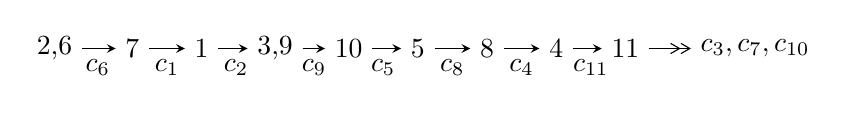
\begin{tikzpicture}[x=25pt, y=7pt]
	% node
	\node (A0) at (-1/8, 0) {2,6};
	\node (A1) at (1, 0) {7};
	\node (A2) at (2, 0) {1};
	\node (A3) at (49/16, 0) {3,9};
	\node (A4) at (33/8, 0) {10};
	\node (A5) at (41/8, 0) {5};
	\node (A6) at (49/8, 0) {8};
	\node (A7) at (57/8, 0) {4};
	\node (A8) at (65/8, 0) {11};
	\node (C1) at (1/2, -1) {$c_{6}$};
	\node (C2) at (3/2, -1) {$c_{1}$};
	\node (C3) at (5/2, -1) {$c_{2}$};
	\node (C4) at (29/8, -1) {$c_{9}$};
	\node (C5) at (37/8, -1) {$c_{5}$};
	\node (C6) at (45/8, -1) {$c_{8}$};
	\node (C7) at (53/8, -1) {$c_{4}$};
	\node (C8) at (61/8, -1) {$c_{11}$};
	\node (A9) at (10, 0) {$c_{3},c_{7},c_{10}$};

	% edge
	\draw[->,>=stealth]	
	(A0) edge (A1) (A1) edge (A2) (A2) edge (A3) (A3) edge (A4) (A4) edge (A5) (A5) edge (A6) (A6) edge (A7) (A7) edge (A8) ;
	\draw[->>,>={angle 60}]	
	(A8) edge (A9);
\end{tikzpicture} \\ 

\end{tabular} \\

\footnotetext{
The image of knot diagram is generated by the software ``\textbf{Draw programme}" developed by Andrew Bartholomew(\url{http://www.layer8.co.uk/maths/draw/index.htm\#Running-draw}), where we modified some parts for our purpose(\url{https://github.com/CATsTAILs/LinksPainter}).
}\phantom \\ \newline 
\centering \textbf{Ideals for irreducible components\footnotemark of $X_{\text{par}}$} 
 
\begin{align*}
I^u_{1}&=\langle 
- u^{19}+2 u^{18}+\cdots+b+1,\;5 u^{19}-11 u^{18}+\cdots+2 a-10,\;u^{20}-3 u^{19}+\cdots-6 u+2\rangle \\
I^u_{2}&=\langle 
- u^{11} a+10 u^{11}+\cdots+2 a-13,\;-2 u^{10} a+u^{11}+\cdots+a^2+1,\\
\phantom{I^u_{2}}&\phantom{= \langle  }u^{12}+u^{11}-3 u^{10}-4 u^9+3 u^8+6 u^7+2 u^6-2 u^5-4 u^4-3 u^3+u^2+2 u+1\rangle \\
I^u_{3}&=\langle 
b+1,\;u^3-2 u^2+2 a+4,\;u^4-2 u^2+2\rangle \\
\\
I^v_{1}&=\langle 
a,\;b-1,\;v+1\rangle \\
\end{align*}
\raggedright * 4 irreducible components of $\dim_{\mathbb{C}}=0$, with total 49 representations.\\
\footnotetext{All coefficients of polynomials are rational numbers. But the coefficients are sometimes approximated in decimal forms when there is not enough margin.}
\newpage
\renewcommand{\arraystretch}{1}
\centering \section*{I. $I^u_{1}= \langle - u^{19}+2 u^{18}+\cdots+b+1,\;5 u^{19}-11 u^{18}+\cdots+2 a-10,\;u^{20}-3 u^{19}+\cdots-6 u+2 \rangle$}
\flushleft \textbf{(i) Arc colorings}\\
\begin{tabular}{m{7pt} m{180pt} m{7pt} m{180pt} }
\flushright $a_{2}=$&$\begin{pmatrix}0\\u\end{pmatrix}$ \\
\flushright $a_{6}=$&$\begin{pmatrix}1\\0\end{pmatrix}$ \\
\flushright $a_{7}=$&$\begin{pmatrix}1\\u^2\end{pmatrix}$ \\
\flushright $a_{1}=$&$\begin{pmatrix}u\\u\end{pmatrix}$ \\
\flushright $a_{3}=$&$\begin{pmatrix}- u^3\\- u^3+u\end{pmatrix}$ \\
\flushright $a_{9}=$&$\begin{pmatrix}-\frac{5}{2} u^{19}+\frac{11}{2} u^{18}+\cdots-11 u+5\\u^{19}-2 u^{18}+\cdots+4 u-1\end{pmatrix}$ \\
\flushright $a_{10}=$&$\begin{pmatrix}-\frac{3}{2} u^{19}+\frac{7}{2} u^{18}+\cdots-7 u+3\\u^{19}-2 u^{18}+\cdots+3 u-1\end{pmatrix}$ \\
\flushright $a_{5}=$&$\begin{pmatrix}-\frac{1}{2} u^{19}+\frac{3}{2} u^{18}+\cdots-3 u+2\\u^{18}- u^{17}+\cdots-2 u+1\end{pmatrix}$ \\
\flushright $a_{8}=$&$\begin{pmatrix}u^6- u^4+1\\u^8-2 u^6+2 u^4\end{pmatrix}$ \\
\flushright $a_{4}=$&$\begin{pmatrix}-\frac{3}{2} u^{19}+\frac{7}{2} u^{18}+\cdots-7 u+3\\- u^{19}+3 u^{18}+\cdots-6 u+3\end{pmatrix}$ \\
\flushright $a_{11}=$&$\begin{pmatrix}u^3\\u^5- u^3+u\end{pmatrix}$\\ \flushright $a_{11}=$&$\begin{pmatrix}u^3\\u^5- u^3+u\end{pmatrix}$\\&\end{tabular}
\flushleft \textbf{(ii) Obstruction class $= -1$}\\~\\
\flushleft \textbf{(iii) Cusp Shapes $= 2 u^{19}-12 u^{17}+6 u^{16}+32 u^{15}-30 u^{14}-34 u^{13}+66 u^{12}-14 u^{11}-58 u^{10}+78 u^9-12 u^8-62 u^7+68 u^6-8 u^5-32 u^4+38 u^3-8 u^2-2 u$}\\~\\
\newpage\renewcommand{\arraystretch}{1}
\flushleft \textbf{(iv) u-Polynomials at the component}\newline \\
\begin{tabular}{m{50pt}|m{274pt}}
Crossings & \hspace{64pt}u-Polynomials at each crossing \\
\hline $$\begin{aligned}c_{1},c_{6}\end{aligned}$$&$\begin{aligned}
&u^{20}-3 u^{19}+\cdots-6 u+2
\end{aligned}$\\
\hline $$\begin{aligned}c_{2}\end{aligned}$$&$\begin{aligned}
&u^{20}+11 u^{19}+\cdots+4 u+4
\end{aligned}$\\
\hline $$\begin{aligned}c_{3},c_{4},c_{5}\\c_{8},c_{9},c_{10}\end{aligned}$$&$\begin{aligned}
&u^{20}+u^{19}+\cdots-2 u-1
\end{aligned}$\\
\hline $$\begin{aligned}c_{7},c_{11}\end{aligned}$$&$\begin{aligned}
&u^{20}-9 u^{19}+\cdots+110 u-22
\end{aligned}$\\
\hline
\end{tabular}\\~\\
\newpage\renewcommand{\arraystretch}{1}
\flushleft \textbf{(v) Riley Polynomials at the component}\newline \\
\begin{tabular}{m{50pt}|m{274pt}}
Crossings & \hspace{64pt}Riley Polynomials at each crossing \\
\hline $$\begin{aligned}c_{1},c_{6}\end{aligned}$$&$\begin{aligned}
&y^{20}-11 y^{19}+\cdots-4 y+4
\end{aligned}$\\
\hline $$\begin{aligned}c_{2}\end{aligned}$$&$\begin{aligned}
&y^{20}-3 y^{19}+\cdots-208 y+16
\end{aligned}$\\
\hline $$\begin{aligned}c_{3},c_{4},c_{5}\\c_{8},c_{9},c_{10}\end{aligned}$$&$\begin{aligned}
&y^{20}-27 y^{19}+\cdots-10 y+1
\end{aligned}$\\
\hline $$\begin{aligned}c_{7},c_{11}\end{aligned}$$&$\begin{aligned}
&y^{20}+17 y^{19}+\cdots-4004 y+484
\end{aligned}$\\
\hline
\end{tabular}\\~\\
\newpage\flushleft \textbf{(vi) Complex Volumes and Cusp Shapes}
$$\begin{array}{c|c|c}  
\text{Solutions to }I^u_{1}& \I (\text{vol} + \sqrt{-1}CS) & \text{Cusp shape}\\
 \hline 
\begin{aligned}
u &= \phantom{-}0.544915 + 0.735723 I \\
a &= -0.396672 - 0.140253 I \\
b &= \phantom{-}1.50718 - 0.07179 I\end{aligned}
 & -8.11263 + 1.41331 I & -12.03617 - 0.10296 I \\ \hline\begin{aligned}
u &= \phantom{-}0.544915 - 0.735723 I \\
a &= -0.396672 + 0.140253 I \\
b &= \phantom{-}1.50718 + 0.07179 I\end{aligned}
 & -8.11263 - 1.41331 I & -12.03617 + 0.10296 I \\ \hline\begin{aligned}
u &= \phantom{-}0.128827 + 0.901492 I \\
a &= -0.623064 - 0.737924 I \\
b &= -1.60887 + 0.30371 I\end{aligned}
 & -14.6659 + 7.5175 I & -13.03534 - 3.27786 I \\ \hline\begin{aligned}
u &= \phantom{-}0.128827 - 0.901492 I \\
a &= -0.623064 + 0.737924 I \\
b &= -1.60887 - 0.30371 I\end{aligned}
 & -14.6659 - 7.5175 I & -13.03534 + 3.27786 I \\ \hline\begin{aligned}
u &= \phantom{-}0.773452 + 0.404695 I \\
a &= \phantom{-}0.591002 - 0.705976 I \\
b &= \phantom{-}0.108607 + 0.523595 I\end{aligned}
 & \phantom{-}0.87704 - 1.78379 I & -2.58390 + 5.68445 I \\ \hline\begin{aligned}
u &= \phantom{-}0.773452 - 0.404695 I \\
a &= \phantom{-}0.591002 + 0.705976 I \\
b &= \phantom{-}0.108607 - 0.523595 I\end{aligned}
 & \phantom{-}0.87704 + 1.78379 I & -2.58390 - 5.68445 I \\ \hline\begin{aligned}
u &= \phantom{-}0.977557 + 0.624357 I \\
a &= -0.48691 + 1.67916 I \\
b &= -1.50584 - 0.14245 I\end{aligned}
 & -9.37386 - 6.54808 I & -13.7315 + 5.5285 I \\ \hline\begin{aligned}
u &= \phantom{-}0.977557 - 0.624357 I \\
a &= -0.48691 - 1.67916 I \\
b &= -1.50584 + 0.14245 I\end{aligned}
 & -9.37386 + 6.54808 I & -13.7315 - 5.5285 I \\ \hline\begin{aligned}
u &= -1.21457\phantom{ +0.000000I} \\
a &= -2.22945\phantom{ +0.000000I} \\
b &= -1.62522\phantom{ +0.000000I}\end{aligned}
 & -14.1194\phantom{ +0.000000I} & -17.9240\phantom{ +0.000000I} \\ \hline\begin{aligned}
u &= -1.145210 + 0.438306 I \\
a &= -0.641824 - 0.515615 I \\
b &= -0.535707 - 0.310794 I\end{aligned}
 & -4.07199 + 2.60865 I & -11.03085 + 0.93775 I\\
 \hline 
 \end{array}$$\newpage$$\begin{array}{c|c|c}  
\text{Solutions to }I^u_{1}& \I (\text{vol} + \sqrt{-1}CS) & \text{Cusp shape}\\
 \hline 
\begin{aligned}
u &= -1.145210 - 0.438306 I \\
a &= -0.641824 + 0.515615 I \\
b &= -0.535707 + 0.310794 I\end{aligned}
 & -4.07199 - 2.60865 I & -11.03085 - 0.93775 I \\ \hline\begin{aligned}
u &= \phantom{-}1.160540 + 0.458172 I \\
a &= -1.261220 + 0.382851 I \\
b &= -0.503696 - 0.478862 I\end{aligned}
 & -3.93117 - 5.51600 I & -10.44810 + 8.22749 I \\ \hline\begin{aligned}
u &= \phantom{-}1.160540 - 0.458172 I \\
a &= -1.261220 - 0.382851 I \\
b &= -0.503696 + 0.478862 I\end{aligned}
 & -3.93117 + 5.51600 I & -10.44810 - 8.22749 I \\ \hline\begin{aligned}
u &= -0.695075\phantom{ +0.000000I} \\
a &= \phantom{-}0.614797\phantom{ +0.000000I} \\
b &= \phantom{-}0.332547\phantom{ +0.000000I}\end{aligned}
 & -0.859562\phantom{ +0.000000I} & -12.8980\phantom{ +0.000000I} \\ \hline\begin{aligned}
u &= -1.280150 + 0.384189 I \\
a &= \phantom{-}2.09625 + 0.60113 I \\
b &= \phantom{-}1.65612 + 0.28210 I\end{aligned}
 & -19.0845 - 3.0881 I & -16.9887 + 0.4542 I \\ \hline\begin{aligned}
u &= -1.280150 - 0.384189 I \\
a &= \phantom{-}2.09625 - 0.60113 I \\
b &= \phantom{-}1.65612 - 0.28210 I\end{aligned}
 & -19.0845 + 3.0881 I & -16.9887 - 0.4542 I \\ \hline\begin{aligned}
u &= \phantom{-}0.058790 + 0.660109 I \\
a &= \phantom{-}0.455681 + 0.359674 I \\
b &= \phantom{-}0.418244 - 0.389912 I\end{aligned}
 & -0.84744 + 1.30386 I & -6.93259 - 5.24353 I \\ \hline\begin{aligned}
u &= \phantom{-}0.058790 - 0.660109 I \\
a &= \phantom{-}0.455681 - 0.359674 I \\
b &= \phantom{-}0.418244 + 0.389912 I\end{aligned}
 & -0.84744 - 1.30386 I & -6.93259 + 5.24353 I \\ \hline\begin{aligned}
u &= \phantom{-}1.236100 + 0.531142 I \\
a &= \phantom{-}2.07408 - 1.71089 I \\
b &= \phantom{-}1.61029 + 0.34268 I\end{aligned}
 & -18.0142 - 12.6981 I & -15.8020 + 6.4148 I \\ \hline\begin{aligned}
u &= \phantom{-}1.236100 - 0.531142 I \\
a &= \phantom{-}2.07408 + 1.71089 I \\
b &= \phantom{-}1.61029 - 0.34268 I\end{aligned}
 & -18.0142 + 12.6981 I & -15.8020 - 6.4148 I\\
 \hline 
 \end{array}$$\newpage\newpage\renewcommand{\arraystretch}{1}
\centering \section*{II. $I^u_{2}= \langle - u^{11} a+10 u^{11}+\cdots+2 a-13,\;-2 u^{10} a+u^{11}+\cdots+a^2+1,\;u^{12}+u^{11}+\cdots+2 u+1 \rangle$}
\flushleft \textbf{(i) Arc colorings}\\
\begin{tabular}{m{7pt} m{180pt} m{7pt} m{180pt} }
\flushright $a_{2}=$&$\begin{pmatrix}0\\u\end{pmatrix}$ \\
\flushright $a_{6}=$&$\begin{pmatrix}1\\0\end{pmatrix}$ \\
\flushright $a_{7}=$&$\begin{pmatrix}1\\u^2\end{pmatrix}$ \\
\flushright $a_{1}=$&$\begin{pmatrix}u\\u\end{pmatrix}$ \\
\flushright $a_{3}=$&$\begin{pmatrix}- u^3\\- u^3+u\end{pmatrix}$ \\
\flushright $a_{9}=$&$\begin{pmatrix}a\\\frac{1}{14} u^{11} a-\frac{5}{7} u^{11}+\cdots-\frac{1}{7} a+\frac{13}{14}\end{pmatrix}$ \\
\flushright $a_{10}=$&$\begin{pmatrix}-\frac{1}{14} u^{11} a-\frac{2}{7} u^{11}+\cdots+\frac{8}{7} a+\frac{1}{14}\\-0.214286 a u^{11}-1.35714 u^{11}+\cdots-0.0714286 a+0.714286\end{pmatrix}$ \\
\flushright $a_{5}=$&$\begin{pmatrix}0.285714 a u^{11}-0.357143 u^{11}+\cdots+0.928571 a+1.21429\\-0.357143 a u^{11}+0.0714286 u^{11}+\cdots+0.214286 a-1.14286\end{pmatrix}$ \\
\flushright $a_{8}=$&$\begin{pmatrix}u^6- u^4+1\\u^8-2 u^6+2 u^4\end{pmatrix}$ \\
\flushright $a_{4}=$&$\begin{pmatrix}-\frac{1}{14} u^{11} a-\frac{2}{7} u^{11}+\cdots+\frac{8}{7} a+\frac{1}{14}\\\frac{1}{14} u^{11} a+\frac{2}{7} u^{11}+\cdots-\frac{1}{7} a-\frac{15}{14}\end{pmatrix}$ \\
\flushright $a_{11}=$&$\begin{pmatrix}u^3\\u^5- u^3+u\end{pmatrix}$\\ \flushright $a_{11}=$&$\begin{pmatrix}u^3\\u^5- u^3+u\end{pmatrix}$\\&\end{tabular}
\flushleft \textbf{(ii) Obstruction class $= -1$}\\~\\
\flushleft \textbf{(iii) Cusp Shapes $= 4 u^{10}-12 u^8-4 u^7+16 u^6+8 u^5-8 u^3-8 u^2-4 u-6$}\\~\\
\newpage\renewcommand{\arraystretch}{1}
\flushleft \textbf{(iv) u-Polynomials at the component}\newline \\
\begin{tabular}{m{50pt}|m{274pt}}
Crossings & \hspace{64pt}u-Polynomials at each crossing \\
\hline $$\begin{aligned}c_{1},c_{6}\end{aligned}$$&$\begin{aligned}
&(u^{12}+u^{11}+\cdots+2 u+1)^{2}
\end{aligned}$\\
\hline $$\begin{aligned}c_{2}\end{aligned}$$&$\begin{aligned}
&(u^{12}+7 u^{11}+\cdots+2 u+1)^{2}
\end{aligned}$\\
\hline $$\begin{aligned}c_{3},c_{4},c_{5}\\c_{8},c_{9},c_{10}\end{aligned}$$&$\begin{aligned}
&u^{24}+u^{23}+\cdots-10 u+5
\end{aligned}$\\
\hline $$\begin{aligned}c_{7},c_{11}\end{aligned}$$&$\begin{aligned}
&(u^{12}+3 u^{11}+\cdots+2 u+1)^{2}
\end{aligned}$\\
\hline
\end{tabular}\\~\\
\newpage\renewcommand{\arraystretch}{1}
\flushleft \textbf{(v) Riley Polynomials at the component}\newline \\
\begin{tabular}{m{50pt}|m{274pt}}
Crossings & \hspace{64pt}Riley Polynomials at each crossing \\
\hline $$\begin{aligned}c_{1},c_{6}\end{aligned}$$&$\begin{aligned}
&(y^{12}-7 y^{11}+\cdots-2 y+1)^{2}
\end{aligned}$\\
\hline $$\begin{aligned}c_{2}\end{aligned}$$&$\begin{aligned}
&(y^{12}-3 y^{11}+\cdots+6 y+1)^{2}
\end{aligned}$\\
\hline $$\begin{aligned}c_{3},c_{4},c_{5}\\c_{8},c_{9},c_{10}\end{aligned}$$&$\begin{aligned}
&y^{24}-21 y^{23}+\cdots-220 y+25
\end{aligned}$\\
\hline $$\begin{aligned}c_{7},c_{11}\end{aligned}$$&$\begin{aligned}
&(y^{12}+13 y^{11}+\cdots+6 y+1)^{2}
\end{aligned}$\\
\hline
\end{tabular}\\~\\
\newpage\flushleft \textbf{(vi) Complex Volumes and Cusp Shapes}
$$\begin{array}{c|c|c}  
\text{Solutions to }I^u_{2}& \I (\text{vol} + \sqrt{-1}CS) & \text{Cusp shape}\\
 \hline 
\begin{aligned}
u &= \phantom{-}0.961384 + 0.208970 I \\
a &= \phantom{-}0.506127 + 0.593369 I \\
b &= \phantom{-}0.915862 - 0.401943 I\end{aligned}
 & -5.02961 - 0.71593 I & -15.9565 + 0.6487 I \\ \hline\begin{aligned}
u &= \phantom{-}0.961384 + 0.208970 I \\
a &= -2.66748 + 1.31736 I \\
b &= -1.242690 - 0.150848 I\end{aligned}
 & -5.02961 - 0.71593 I & -15.9565 + 0.6487 I \\ \hline\begin{aligned}
u &= \phantom{-}0.961384 - 0.208970 I \\
a &= \phantom{-}0.506127 - 0.593369 I \\
b &= \phantom{-}0.915862 + 0.401943 I\end{aligned}
 & -5.02961 + 0.71593 I & -15.9565 - 0.6487 I \\ \hline\begin{aligned}
u &= \phantom{-}0.961384 - 0.208970 I \\
a &= -2.66748 - 1.31736 I \\
b &= -1.242690 + 0.150848 I\end{aligned}
 & -5.02961 + 0.71593 I & -15.9565 - 0.6487 I \\ \hline\begin{aligned}
u &= -0.958024 + 0.460561 I \\
a &= -0.002595 + 0.970301 I \\
b &= \phantom{-}0.317703 - 0.537023 I\end{aligned}
 & -3.21312 + 4.24921 I & -9.82351 - 6.98310 I \\ \hline\begin{aligned}
u &= -0.958024 + 0.460561 I \\
a &= -1.13256 - 1.76796 I \\
b &= -1.233460 + 0.149435 I\end{aligned}
 & -3.21312 + 4.24921 I & -9.82351 - 6.98310 I \\ \hline\begin{aligned}
u &= -0.958024 - 0.460561 I \\
a &= -0.002595 - 0.970301 I \\
b &= \phantom{-}0.317703 + 0.537023 I\end{aligned}
 & -3.21312 - 4.24921 I & -9.82351 + 6.98310 I \\ \hline\begin{aligned}
u &= -0.958024 - 0.460561 I \\
a &= -1.13256 + 1.76796 I \\
b &= -1.233460 - 0.149435 I\end{aligned}
 & -3.21312 - 4.24921 I & -9.82351 + 6.98310 I \\ \hline\begin{aligned}
u &= -0.049813 + 0.844037 I \\
a &= -1.205190 + 0.406247 I \\
b &= -1.51479 - 0.10395 I\end{aligned}
 & -7.33005 - 3.01307 I & -11.36825 + 2.63251 I \\ \hline\begin{aligned}
u &= -0.049813 + 0.844037 I \\
a &= \phantom{-}0.190483 - 0.652317 I \\
b &= \phantom{-}0.619350 + 0.907491 I\end{aligned}
 & -7.33005 - 3.01307 I & -11.36825 + 2.63251 I\\
 \hline 
 \end{array}$$\newpage$$\begin{array}{c|c|c}  
\text{Solutions to }I^u_{2}& \I (\text{vol} + \sqrt{-1}CS) & \text{Cusp shape}\\
 \hline 
\begin{aligned}
u &= -0.049813 - 0.844037 I \\
a &= -1.205190 - 0.406247 I \\
b &= -1.51479 + 0.10395 I\end{aligned}
 & -7.33005 + 3.01307 I & -11.36825 - 2.63251 I \\ \hline\begin{aligned}
u &= -0.049813 - 0.844037 I \\
a &= \phantom{-}0.190483 + 0.652317 I \\
b &= \phantom{-}0.619350 - 0.907491 I\end{aligned}
 & -7.33005 + 3.01307 I & -11.36825 - 2.63251 I \\ \hline\begin{aligned}
u &= \phantom{-}1.238640 + 0.435356 I \\
a &= -0.178745 + 0.729514 I \\
b &= -0.704482 + 0.930610 I\end{aligned}
 & -11.20510 - 1.48234 I & -15.1526 + 0.6754 I \\ \hline\begin{aligned}
u &= \phantom{-}1.238640 + 0.435356 I \\
a &= \phantom{-}2.56411 - 0.92305 I \\
b &= \phantom{-}1.55418 - 0.05622 I\end{aligned}
 & -11.20510 - 1.48234 I & -15.1526 + 0.6754 I \\ \hline\begin{aligned}
u &= \phantom{-}1.238640 - 0.435356 I \\
a &= -0.178745 - 0.729514 I \\
b &= -0.704482 - 0.930610 I\end{aligned}
 & -11.20510 + 1.48234 I & -15.1526 - 0.6754 I \\ \hline\begin{aligned}
u &= \phantom{-}1.238640 - 0.435356 I \\
a &= \phantom{-}2.56411 + 0.92305 I \\
b &= \phantom{-}1.55418 + 0.05622 I\end{aligned}
 & -11.20510 + 1.48234 I & -15.1526 - 0.6754 I \\ \hline\begin{aligned}
u &= -1.228550 + 0.484706 I \\
a &= -1.41739 - 0.27157 I \\
b &= -0.584122 + 0.976162 I\end{aligned}
 & -10.84800 + 7.80134 I & -14.3661 - 5.6398 I \\ \hline\begin{aligned}
u &= -1.228550 + 0.484706 I \\
a &= \phantom{-}2.49284 + 1.50692 I \\
b &= \phantom{-}1.54701 - 0.14731 I\end{aligned}
 & -10.84800 + 7.80134 I & -14.3661 - 5.6398 I \\ \hline\begin{aligned}
u &= -1.228550 - 0.484706 I \\
a &= -1.41739 + 0.27157 I \\
b &= -0.584122 - 0.976162 I\end{aligned}
 & -10.84800 - 7.80134 I & -14.3661 + 5.6398 I \\ \hline\begin{aligned}
u &= -1.228550 - 0.484706 I \\
a &= \phantom{-}2.49284 - 1.50692 I \\
b &= \phantom{-}1.54701 + 0.14731 I\end{aligned}
 & -10.84800 - 7.80134 I & -14.3661 + 5.6398 I\\
 \hline 
 \end{array}$$\newpage$$\begin{array}{c|c|c}  
\text{Solutions to }I^u_{2}& \I (\text{vol} + \sqrt{-1}CS) & \text{Cusp shape}\\
 \hline 
\begin{aligned}
u &= -0.463636 + 0.458719 I \\
a &= \phantom{-}1.49987 + 0.51998 I \\
b &= -0.312209 - 0.212773 I\end{aligned}
 & -1.85256 - 0.35310 I & -5.33308 + 0.62981 I \\ \hline\begin{aligned}
u &= -0.463636 + 0.458719 I \\
a &= -0.149462 - 0.021454 I \\
b &= \phantom{-}1.137650 + 0.055627 I\end{aligned}
 & -1.85256 - 0.35310 I & -5.33308 + 0.62981 I \\ \hline\begin{aligned}
u &= -0.463636 - 0.458719 I \\
a &= \phantom{-}1.49987 - 0.51998 I \\
b &= -0.312209 + 0.212773 I\end{aligned}
 & -1.85256 + 0.35310 I & -5.33308 - 0.62981 I \\ \hline\begin{aligned}
u &= -0.463636 - 0.458719 I \\
a &= -0.149462 + 0.021454 I \\
b &= \phantom{-}1.137650 - 0.055627 I\end{aligned}
 & -1.85256 + 0.35310 I & -5.33308 - 0.62981 I\\
 \hline 
 \end{array}$$\newpage\newpage\renewcommand{\arraystretch}{1}
\centering \section*{III. $I^u_{3}= \langle b+1,\;u^3-2 u^2+2 a+4,\;u^4-2 u^2+2 \rangle$}
\flushleft \textbf{(i) Arc colorings}\\
\begin{tabular}{m{7pt} m{180pt} m{7pt} m{180pt} }
\flushright $a_{2}=$&$\begin{pmatrix}0\\u\end{pmatrix}$ \\
\flushright $a_{6}=$&$\begin{pmatrix}1\\0\end{pmatrix}$ \\
\flushright $a_{7}=$&$\begin{pmatrix}1\\u^2\end{pmatrix}$ \\
\flushright $a_{1}=$&$\begin{pmatrix}u\\u\end{pmatrix}$ \\
\flushright $a_{3}=$&$\begin{pmatrix}- u^3\\- u^3+u\end{pmatrix}$ \\
\flushright $a_{9}=$&$\begin{pmatrix}-\frac{1}{2} u^3+u^2-2\\-1\end{pmatrix}$ \\
\flushright $a_{10}=$&$\begin{pmatrix}\frac{1}{2} u^3+u^2-2\\u^3- u-1\end{pmatrix}$ \\
\flushright $a_{5}=$&$\begin{pmatrix}-\frac{1}{2} u^3+u^2-1\\-1\end{pmatrix}$ \\
\flushright $a_{8}=$&$\begin{pmatrix}-1\\0\end{pmatrix}$ \\
\flushright $a_{4}=$&$\begin{pmatrix}-\frac{1}{2} u^3+u^2-2\\-1\end{pmatrix}$ \\
\flushright $a_{11}=$&$\begin{pmatrix}u^3\\u^3- u\end{pmatrix}$\\ \flushright $a_{11}=$&$\begin{pmatrix}u^3\\u^3- u\end{pmatrix}$\\&\end{tabular}
\flushleft \textbf{(ii) Obstruction class $= 1$}\\~\\
\flushleft \textbf{(iii) Cusp Shapes $= 4 u^2-20$}\\~\\
\newpage\renewcommand{\arraystretch}{1}
\flushleft \textbf{(iv) u-Polynomials at the component}\newline \\
\begin{tabular}{m{50pt}|m{274pt}}
Crossings & \hspace{64pt}u-Polynomials at each crossing \\
\hline $$\begin{aligned}c_{1},c_{6}\end{aligned}$$&$\begin{aligned}
&u^4-2 u^2+2
\end{aligned}$\\
\hline $$\begin{aligned}c_{2}\end{aligned}$$&$\begin{aligned}
&(u^2+2 u+2)^2
\end{aligned}$\\
\hline $$\begin{aligned}c_{3},c_{8}\end{aligned}$$&$\begin{aligned}
&(u-1)^4
\end{aligned}$\\
\hline $$\begin{aligned}c_{4},c_{5},c_{9}\\c_{10}\end{aligned}$$&$\begin{aligned}
&(u+1)^4
\end{aligned}$\\
\hline $$\begin{aligned}c_{7},c_{11}\end{aligned}$$&$\begin{aligned}
&u^4+2 u^2+2
\end{aligned}$\\
\hline
\end{tabular}\\~\\
\newpage\renewcommand{\arraystretch}{1}
\flushleft \textbf{(v) Riley Polynomials at the component}\newline \\
\begin{tabular}{m{50pt}|m{274pt}}
Crossings & \hspace{64pt}Riley Polynomials at each crossing \\
\hline $$\begin{aligned}c_{1},c_{6}\end{aligned}$$&$\begin{aligned}
&(y^2-2 y+2)^2
\end{aligned}$\\
\hline $$\begin{aligned}c_{2}\end{aligned}$$&$\begin{aligned}
&(y^2+4)^2
\end{aligned}$\\
\hline $$\begin{aligned}c_{3},c_{4},c_{5}\\c_{8},c_{9},c_{10}\end{aligned}$$&$\begin{aligned}
&(y-1)^4
\end{aligned}$\\
\hline $$\begin{aligned}c_{7},c_{11}\end{aligned}$$&$\begin{aligned}
&(y^2+2 y+2)^2
\end{aligned}$\\
\hline
\end{tabular}\\~\\
\newpage\flushleft \textbf{(vi) Complex Volumes and Cusp Shapes}
$$\begin{array}{c|c|c}  
\text{Solutions to }I^u_{3}& \I (\text{vol} + \sqrt{-1}CS) & \text{Cusp shape}\\
 \hline 
\begin{aligned}
u &= \phantom{-}1.098680 + 0.455090 I \\
a &= -1.321800 + 0.223113 I \\
b &= -1.00000\phantom{ +0.000000I}\end{aligned}
 & -5.75727 - 3.66386 I & -16.0000 + 4.0000 I \\ \hline\begin{aligned}
u &= \phantom{-}1.098680 - 0.455090 I \\
a &= -1.321800 - 0.223113 I \\
b &= -1.00000\phantom{ +0.000000I}\end{aligned}
 & -5.75727 + 3.66386 I & -16.0000 - 4.0000 I \\ \hline\begin{aligned}
u &= -1.098680 + 0.455090 I \\
a &= -0.67820 - 1.77689 I \\
b &= -1.00000\phantom{ +0.000000I}\end{aligned}
 & -5.75727 + 3.66386 I & -16.0000 - 4.0000 I \\ \hline\begin{aligned}
u &= -1.098680 - 0.455090 I \\
a &= -0.67820 + 1.77689 I \\
b &= -1.00000\phantom{ +0.000000I}\end{aligned}
 & -5.75727 - 3.66386 I & -16.0000 + 4.0000 I\\
 \hline 
 \end{array}$$\newpage\newpage\renewcommand{\arraystretch}{1}
\centering \section*{IV. $I^v_{1}= \langle a,\;b-1,\;v+1 \rangle$}
\flushleft \textbf{(i) Arc colorings}\\
\begin{tabular}{m{7pt} m{180pt} m{7pt} m{180pt} }
\flushright $a_{2}=$&$\begin{pmatrix}-1\\0\end{pmatrix}$ \\
\flushright $a_{6}=$&$\begin{pmatrix}1\\0\end{pmatrix}$ \\
\flushright $a_{7}=$&$\begin{pmatrix}1\\0\end{pmatrix}$ \\
\flushright $a_{1}=$&$\begin{pmatrix}-1\\0\end{pmatrix}$ \\
\flushright $a_{3}=$&$\begin{pmatrix}-1\\0\end{pmatrix}$ \\
\flushright $a_{9}=$&$\begin{pmatrix}0\\1\end{pmatrix}$ \\
\flushright $a_{10}=$&$\begin{pmatrix}-1\\1\end{pmatrix}$ \\
\flushright $a_{5}=$&$\begin{pmatrix}1\\-1\end{pmatrix}$ \\
\flushright $a_{8}=$&$\begin{pmatrix}1\\0\end{pmatrix}$ \\
\flushright $a_{4}=$&$\begin{pmatrix}0\\-1\end{pmatrix}$ \\
\flushright $a_{11}=$&$\begin{pmatrix}-1\\0\end{pmatrix}$\\ \flushright $a_{11}=$&$\begin{pmatrix}-1\\0\end{pmatrix}$\\&\end{tabular}
\flushleft \textbf{(ii) Obstruction class $= 1$}\\~\\
\flushleft \textbf{(iii) Cusp Shapes $= -12$}\\~\\
\newpage\renewcommand{\arraystretch}{1}
\flushleft \textbf{(iv) u-Polynomials at the component}\newline \\
\begin{tabular}{m{50pt}|m{274pt}}
Crossings & \hspace{64pt}u-Polynomials at each crossing \\
\hline $$\begin{aligned}c_{1},c_{2},c_{6}\\c_{7},c_{11}\end{aligned}$$&$\begin{aligned}
&u
\end{aligned}$\\
\hline $$\begin{aligned}c_{3},c_{8}\end{aligned}$$&$\begin{aligned}
&u+1
\end{aligned}$\\
\hline $$\begin{aligned}c_{4},c_{5},c_{9}\\c_{10}\end{aligned}$$&$\begin{aligned}
&u-1
\end{aligned}$\\
\hline
\end{tabular}\\~\\
\newpage\renewcommand{\arraystretch}{1}
\flushleft \textbf{(v) Riley Polynomials at the component}\newline \\
\begin{tabular}{m{50pt}|m{274pt}}
Crossings & \hspace{64pt}Riley Polynomials at each crossing \\
\hline $$\begin{aligned}c_{1},c_{2},c_{6}\\c_{7},c_{11}\end{aligned}$$&$\begin{aligned}
&y
\end{aligned}$\\
\hline $$\begin{aligned}c_{3},c_{4},c_{5}\\c_{8},c_{9},c_{10}\end{aligned}$$&$\begin{aligned}
&y-1
\end{aligned}$\\
\hline
\end{tabular}\\~\\
\newpage\flushleft \textbf{(vi) Complex Volumes and Cusp Shapes}
$$\begin{array}{c|c|c}  
\text{Solutions to }I^v_{1}& \I (\text{vol} + \sqrt{-1}CS) & \text{Cusp shape}\\
 \hline 
\begin{aligned}
v &= -1.00000\phantom{ +0.000000I} \\
a &= \phantom{-0.000000 } 0 \\
b &= \phantom{-}1.00000\phantom{ +0.000000I}\end{aligned}
 & -3.28987\phantom{ +0.000000I} & -12.0000\phantom{ +0.000000I}\\
 \hline 
 \end{array}$$\newpage
\newpage\renewcommand{\arraystretch}{1}
\centering \section*{ V. u-Polynomials}
\begin{tabular}{m{50pt}|m{274pt}}
Crossings & \hspace{64pt}u-Polynomials at each crossing \\
\hline $$\begin{aligned}c_{1},c_{6}\end{aligned}$$&$\begin{aligned}
&u(u^4-2 u^2+2)(u^{12}+u^{11}+\cdots+2 u+1)^{2}(u^{20}-3 u^{19}+\cdots-6 u+2)
\end{aligned}$\\
\hline $$\begin{aligned}c_{2}\end{aligned}$$&$\begin{aligned}
&u(u^2+2 u+2)^2(u^{12}+7 u^{11}+\cdots+2 u+1)^{2}\\
&\cdot(u^{20}+11 u^{19}+\cdots+4 u+4)
\end{aligned}$\\
\hline $$\begin{aligned}c_{3},c_{8}\end{aligned}$$&$\begin{aligned}
&((u-1)^4)(u+1)(u^{20}+u^{19}+\cdots-2 u-1)(u^{24}+u^{23}+\cdots-10 u+5)
\end{aligned}$\\
\hline $$\begin{aligned}c_{4},c_{5},c_{9}\\c_{10}\end{aligned}$$&$\begin{aligned}
&(u-1)(u+1)^4(u^{20}+u^{19}+\cdots-2 u-1)(u^{24}+u^{23}+\cdots-10 u+5)
\end{aligned}$\\
\hline $$\begin{aligned}c_{7},c_{11}\end{aligned}$$&$\begin{aligned}
&u(u^4+2 u^2+2)(u^{12}+3 u^{11}+\cdots+2 u+1)^{2}\\
&\cdot(u^{20}-9 u^{19}+\cdots+110 u-22)
\end{aligned}$\\
\hline
\end{tabular}\newpage\renewcommand{\arraystretch}{1}
\centering \section*{ VI. Riley Polynomials}
\begin{tabular}{m{50pt}|m{274pt}}
Crossings & \hspace{64pt}Riley Polynomials at each crossing \\
\hline $$\begin{aligned}c_{1},c_{6}\end{aligned}$$&$\begin{aligned}
&y(y^2-2 y+2)^2(y^{12}-7 y^{11}+\cdots-2 y+1)^{2}\\
&\cdot(y^{20}-11 y^{19}+\cdots-4 y+4)
\end{aligned}$\\
\hline $$\begin{aligned}c_{2}\end{aligned}$$&$\begin{aligned}
&y(y^2+4)^2(y^{12}-3 y^{11}+\cdots+6 y+1)^{2}(y^{20}-3 y^{19}+\cdots-208 y+16)
\end{aligned}$\\
\hline $$\begin{aligned}c_{3},c_{4},c_{5}\\c_{8},c_{9},c_{10}\end{aligned}$$&$\begin{aligned}
&((y-1)^5)(y^{20}-27 y^{19}+\cdots-10 y+1)(y^{24}-21 y^{23}+\cdots-220 y+25)
\end{aligned}$\\
\hline $$\begin{aligned}c_{7},c_{11}\end{aligned}$$&$\begin{aligned}
&y(y^2+2 y+2)^2(y^{12}+13 y^{11}+\cdots+6 y+1)^{2}\\
&\cdot(y^{20}+17 y^{19}+\cdots-4004 y+484)
\end{aligned}$\\
\hline
\end{tabular}
\vskip 2pc
\end{document}